\subsubsubsubsection{Lane Decorator}
\begin{figure}[h]
\centering
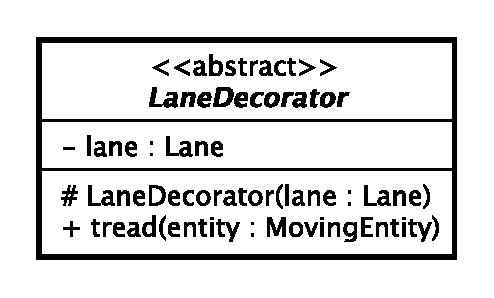
\includegraphics[scale=0.6,keepaspectratio]{images/solution/lane_decorator.eps}
\caption{\pReactiveComponentLaneDecoration::LaneDecorator}
\label{fig:sd-app-lane_decorator}
\end{figure}
\FloatBarrier
\begin{itemize}
  \item \textbf{\descr} \\
    It represents the abstract decorator which enable to compose togheter several
behaviours on the top of a lane component. 
  \item \textbf{\attrs}
  \begin{itemize}
    \item \texttt{lane: Lane} \\
The lane to decorate.
  \end{itemize}
  \item \textbf{\ops}
   \begin{itemize} 
   \item[\#] \texttt{LaneDecorator(lane: Lane)} \\
Creates a lane decorator with a specific lane.
    \item[+] \texttt{tread(entity: MovingEntity)} \\
Decorates the standard behaviour of the lane.  
  \end{itemize}
\end{itemize}
